\begin{figure}
    \centering
    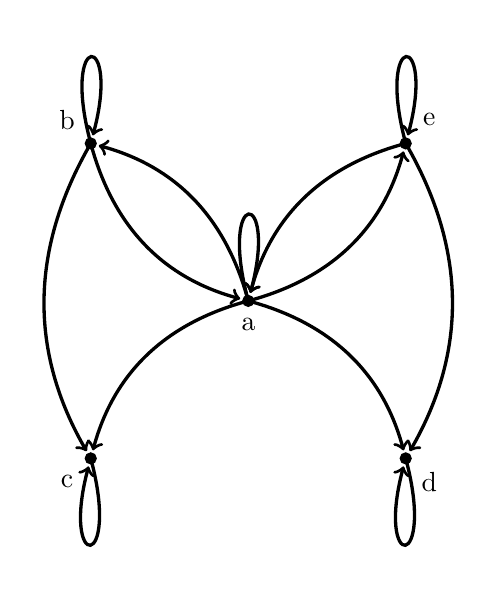
\begin{tikzpicture}

%% vertices
\draw[fill=black] (2,2) circle (2pt);   %% a
\draw[fill=black] (0,4) circle (2pt);   %% b
\draw[fill=black] (0,0) circle (2pt);   %% c
\draw[fill=black] (4,0) circle (2pt);   %% d
\draw[fill=black] (4,4) circle (2pt);   %% e

%% vertex labels
\node at (2,1.7) {a};
\node at (-0.3,4.3) {b};
\node at (-0.3,-0.3) {c};
\node at (4.3,-0.3) {d};
\node at (4.3,4.3) {e};

%%% edges
\draw[-{>[sep=3pt]}, very thick] (2,2) to [loop above, min distance=1.5cm] (2,2);     %% aa
\draw[-{>[sep=3pt]}, very thick] (2,2) to [bend right] (0,4);     %% ab
\draw[-{>[sep=3pt]}, very thick] (0,4) to [bend right] (2,2);     %% ba
\draw[-{>[sep=3pt]}, very thick] (0,4) to [loop above, min distance=1.5cm] (0,4);     %% bb
\draw[-{>[sep=3pt]}, very thick] (2,2) to [bend right] (4,4); %% ae
\draw[-{>[sep=3pt]}, very thick] (4,4) to [bend right] (2,2); %% ea
\draw[-{>[sep=3pt]}, very thick] (4,4) to [loop above, min distance=1.5cm] (4,4);     %% ee
\draw[-{>[sep=3pt]}, very thick] (2,2) to [bend right] (0,0);     %% ac
\draw[-{>[sep=3pt]}, very thick] (2,2) to [bend left] (4,0);     %% ad
\draw[-{>[sep=3pt]}, very thick] (0,4) to [bend right] (0,0);     %% bc
\draw[-{>[sep=3pt]}, very thick] (4,4) to [bend left] (4,0);     %% ed
\draw[-{>[sep=3pt]}, very thick] (0,0) to [loop below, min distance=1.5cm] (0,0);%%cc
\draw[-{>[sep=3pt]}, very thick] (4,0) to [loop below, min distance=1.5cm] (4,0);%%dd
    \end{tikzpicture}
    \label{q4-a}
    \caption{Graph in question 5}
\end{figure}